
%\documentclass[paper]{geophysics}
\documentclass[manuscript,revised]{geophysics}
\usepackage{amsmath,amssymb}

% An example of defining macros
\newcommand{\rs}[1]{\mathstrut\mbox{\scriptsize\rm #1}}
\newcommand{\rr}[1]{\mbox{\rm #1}}

\begin{document}

\title{3D inversion for estimating total magnetization direction using equivalent layer technique}

\renewcommand{\thefootnote}{\fnsymbol{footnote}} 

\ms{GEO-2018XXXX} % manuscript number

\address{
\footnotemark[2] Observat\'orio Nacional, Rio de Janeiro, Brazil\\
\footnotemark[1] Corresponding author: decoluisreis@gmail.com}
\author{Andr\'e L. A. Reis\footnotemark[2] \footnotemark[1], Vanderlei C. Oliveira Jr.\footnotemark[2] and Val\'eria C. F. Barbosa \footnotemark[2]}

%\footer{Example}
\lefthead{Reis, A.L.A. \& Oliveira Jr, V.C. \& Barbosa, V. C. F.}
\righthead{Determining total magnetization direction}

\maketitle


\begin{abstract}
We developed a new method for estimating the total magnetization direction of magnetic sources based on equivalent-layer technique using total-field anomaly data. This approach does not impose strong information either about the shape or about the depth of the sources, and does not require a regularly spaced data. Usually, the equivalent-layer technique is used for processing total-field anomaly data by estimating a 2D magnetic-moment distribution over a fictitional layer composed by dipoles below the observation plane. When the magnetization direction of equivalent sources is almost the same as the true body, the estimated magnetic property over the layer is all positive. Iteratively, the proposed method imposes zeroth-order Tikhonov regularization and positivity constraint on the estimated magnetic moment over the layer and estimate the magnetization direction of the geological sources. Mathematically, the algorithm solves least-squares problems in two steps: the first one solves a linear inverse problem for estimating a 2D magnetic-moment distribution within the equivalent layer and the second solves a nonlinear inverse problem for magnetization direction of the magnetized sources. We test the methodology by applying to synthetic data for different geological scenarios, and the results show that the method can be a powerful tool for estimating the magnetization direction of a set of bodies. Tests on field data from Goias Alkaline Province (GAP), center of Brazil, over Montes Claros complex suggests intrusions with remarkable strong remanent magnetization, in agreement with the current literature for this region. 
\end{abstract}
%\section{Introduction}

%% The importance of magnetization direction and techniques
Most of  magnetic methods require knowledge of the magnetization direction, otherwise 
they yield unsatisfactory interpretations of the exploration targets. This fact has 
been propelled the development of several techniques for estimating magnetization 
direction over the last 50 years. The strategies for estimating this quantity can be 
divided into two main groups. The first one comprises the methods which presume a prior 
information about the shape of geological sources. The iterative method presented by 
\cite{bhattacharyya1966} presumed that the magnetic source has a rectangular prismatic shape. 
\cite{emilia_massey_1974} approximated a seamount by a set of stacked 
prisms with uniform magnetization direction and variable magnetization intensity. 
\cite{parker_etal_1987} approximated the geometry of a seamount by using a 
covering of triangular facets and estimate the internal magnetization closest to 
a uniform solution.
\cite{medeiros_silva_1995} presented a method that estimates the total magnetization 
direction and the spatial orientation of an isolated source having three othogonal planes of 
symmetry. 
\cite{kubota2005} also approximated a seamount by a set of juxtaposed prisms, but estimate a 
magnetization direction for each one. 
Finally, \cite{oliveirajr_etal_2015} approximated the magnetic sources by spherical bodies with 
known centers for estimating their magnetization directions. 
The second group is formed by methods which do not presume any information about the shape of the 
magnetic sources. \cite{fedi_etal_1994}, for example, proposed a method that determines the best 
magnetization direction among a set a tentative values used to perform 
successive reductions-to-the-pole on Fourier domain. 
\cite{phillips2005} used the Helbig's integral for estimating the components of the magnetic-moment vector. 
\cite{tontini_pedersen_2008} extended the Phillips' method by using the same Helbig's integral 
to estimate the magnetization direction and its magnitude, also providing information about the position 
of the center of magnetization distribution. \cite{lelievre_oldenburg_2009} developed a method for estimating 
the magnetization direction in complex geological scenarios. Their method approximates the subsurface 
by a grid of juxtaposed prisms and estimates the components of the magnetization vector for each prism.
In addition, there are methods based on the correlation of potential-field quantities \citep[e.g.,][]{dannemiller_li_2006,gerovska_etal_2009,liu_etal_2015,zhang_etal_2018}.

%%The equivalent layer 
Estimating the magnetization direction is extremely important not only for interpretation, 
but also for processing the total-field anomaly data. One technique in spatial domain 
commonly used for processing potential-field data is the equivalent layer. It was first introduced 
in exploration geophysics by \cite{dampney1969} and \cite{emilia_massey_1974} for processing 
gravity and magnetic data, respectively. After these pioneer works, this technique has been widely 
used for computing interpolation \citep{cordell_1992, mendonca-silva_1994, barnes-lumley_2011, siqueira_etal_2017}, 
upward (or downward) continuation  \citep{hansen-miyazaki_1984, li-oldenburg_2010}, reduction to the pole 
\citep{silva_1986, leao-silva_1989, guspi-novara_2009, oliveirajr-etal_2013}, the amplitude of 
anomalous field \citep{li_li_2014} and for denoising gradient data \citep{martinez_li_2016}. 
The equivalent-layer technique consists in approximating the observed data by that produced by a 
layer of discrete sources (e.g., prisms, dipoles or point masses), which are commonly known as 
equivalent sources. The data produced by this fictitious layer (the equivalent layer) are commonly
called predicted data.

%%  positivity constraints 
In scanning magnetic microscopy, the equivalent-layer technique is generally used for interpreting 
the magnetic-moment distribution whithin thin planar sections of rock samples. Notice that, in this case, 
the equivalent layer resembles the true source (a thin section of rock). 
\cite{weiss2007} presented one of the first works using the equivalent-layer technique in scanning magnetic microscopy.
They pointed out without proof that the estimated magnetic-moment distribution on the layer is all-positive if 
the magnetization direction of the equivalent sources is equal to that used for artificially magnetizing the rock sample. 
\cite{baratchart2013} showed mathematically that, assuming a uniform magnetization direction within the thin section, 
the inverse problem of estimating the magnetic-moment distribution has uniqueness. 
\cite{lima2013} proposed a method on the frequency domain to investigate solutions having a uniform magnetization 
direction equal to that of a thin section of geological sample. They show empirically 
that, in this case, the estimated magnetic-moment distribution on the layer is entirely positive. 

In the geophysical exploration, the equivalent-layer technique is predominantly used for processing potential-field data. 
Under this perspective, there is no relationship between the physical-property distribution on the equivalent layer 
and the true geological sources. Hence, the layer is just a mathematical abstraction devoid of geological meaning. 
Few authors in geophysical exploration literature have been addressed the use of the equivalent-layer technique for interpreting
the geological sources. \cite{pedersen1991}, for example, discussed the relationship between potential field and equivalent source. 
\cite{medeiros_silva1996} and \cite{silvadias_etal_2010} estimated an apparent-magnetization map on a layer by using Tikhonov and 
entropic regularizations respectively. \cite{siqueira_etal_2017} established a relationship between the excess of mass estimated 
over the equivalent layer and the true one. \cite{li_etal_2014} proved, by using an approach in the Fourier domain, 
the existence of an all-positive magnetic-moment distribution over the layer and use this to overcome the low-latitude instability. 
However, these authors considered only the particular case in which the magnetic sources have a purely induced magnetization.

%% Joining techniques for estimating the magnetization direction 
Here, we prove mathematically that the all-positive magnetic-moment distribution within an equivalent layer exists even in the 
presence of remanent magnetization of the true geological sources. This all-positive magnetic-moment distribution holds true for 
all cases in which the magnetization direction of the equivalent sources has the same direction as that of the true geological sources, 
regardless of whether the magnetization of the true sources is purely induced or not. Grounded on this generalized positivity constraint, 
we present a new iterative method that uses the equivalent-layer technique for estimating the uniform magnetization direction of 
arbitrary sources by inverting total-field anomaly data. Our method does not presume any information about the shape of the sources. 
At each iteration, our method solves (1) a linear inverse problem, subjected to a positivity constraint, for estimating the magnetic-moment 
distribution within a planar equivalent layer of dipoles, and (2) a non-linear inverse problem for estimating the uniform magnetization 
direction of the equivalent sources. Tests with synthetic data generated by different geological scenarios show that the estimated magnetization
direction converges to that of the true sources. We also applied our method to field data from the Goi{\' a}s alkaline province (GAP), 
over the Montes Claros complex, center of Brazil. Our result is in agreement with that obtained independently by \cite{zhang_etal_2018} 
at the same area, suggests the presence of a remarkable remanent magnetization and shows the good performance of our method in interpreting 
a complex geological scenario.

\section{Methodology}
\label{sec:methodology}

% % Explaining the continuous magnetic equivalent layer  

Considering a Cartesian coordinate system with $x$-, $y$- and $z$-axis being oriented to north, east and downward, respectively. Let $\Delta T_i \equiv \Delta T (x_i,y_i,z_i)$ be the total field anomaly, at the $i$-th position $(x_i,y_i,z_i)$, produced by a continuos layer located below the observation plane on the depth $z_c$, where $z_c > z_i$, and $p(x',y',z_c)$ is the distribution of magnetic dipoles per unit area over the layer surface. In this case, the total field anomaly produced by this continuous layer is given by the equation 

\begin{equation}
\Delta T_i = \int \limits_{-\infty}^{+\infty } \int \limits_{-\infty}^{+\infty }  p(x',y',z_c)  [\gamma_m \hat{\mathbf{F}}_0^T \mathbf{H} \,\hat{\mathbf{h}}(\mathbf{q})] dx' \,dy',
\label{eq:continuous_layer}
\end{equation}
where $\gamma_m$ is a constant proportional to the vaccum permeability, $\hat{\mathbf{F}}_0$ is a unit vector with the same direction of the geomagnetic field $\mathbf{F}_0$ and $\mathbf{H}$ is a $3 \times 3$ matrix equal to  

 \begin{equation}
   \mathbf{H} =
   \left[ \begin{array}{ccc}
   \partial_{xx} \phi & \partial_{xy} \phi &\partial_{xz} \phi \\  \partial_{yx} \phi & \partial_{yy} \phi &\partial_{yz} \phi \\  \partial_{zx} \phi &\partial_{zy}\phi  & \partial_{zz} \phi    
   \end{array} \right] ,
   \label{eq:H}
 \end{equation}
where $\partial_{\alpha \beta}\phi$, $\alpha = x, y, z$, $\beta = x, y, z$, is the second derivative of the function 

\begin{equation}
   \phi (x-x', y-y', z-z_c) = \frac{1}{r} ,
   \label{eq:phi}
 \end{equation}
where $r = [(x-x')^2 + (y-y')^2 + (z-z_c)^2]^{1/2}$ and $\hat{\mathbf{h}}(\mathbf{q})$ is a unit vector with the
magnetization direction of the layer that depends on the vector $\mathbf{q}$ given by 

 \begin{equation}
   \mathbf{q} =
   \left[ \begin{array}{c}
   i  \\ 
   d     
   \end{array} \right] ,
   \label{eq:q_vector}
 \end{equation}
 where $i$ and $d$ is the inclination and declination, respectively.

% % Formulating foward problem 

According the theory, we can reproduce a set of $N$ observed total field anomaly produced by a 3D magnetic source using a bidimensional physical-property distribution. In practical situations, the equivalent layer is composed by a set of $M$ equivalent sources distributed with a constant depth $h$ below the observation plane. It is worth pointing out that, in this work, the equivalent source is represented by a dipole with unit volume. For this reason, the vector $\mathbf{p}$ is the \textit{M}-dimensional vector defined as parameter vector, whose $j$th element is the magnetic intensity of the $j$th equivalent source, and the vector $\mathbf{q}$ contains the inclination and the declination of each equivalent dipole. By discretizing the integrand of equation \ref{eq:continuous_layer} in a set of points $(x_j,y_j,z_c)$, $j = 1, \ldots, M$, the integral can be given by

\begin{equation}
\Delta T_i (\mathbf{p},\mathbf{q})   = \sum_{j=1}^{M} p_j g_{ij} (\mathbf{q})
\label{eq:tfa_pred_pos_i}
\end{equation}    
where $p_j$ is the magnetic moment of $j$th equivalent source and 

\begin{equation}
g_{ij} (\mathbf{q})  = \gamma_m \hat{\mathbf{F}}_0^T \mathbf{H}_{ij} \hat{\mathbf{h}}(\mathbf{q})
\label{eq:g_ij}
\end{equation}
is a harmonic function that depends on the direction $\mathbf{q}$ of the dipole and the matrix $\mathbf{H}_{ij}$ is formed by the second derivatives of a function $\phi_{ij}$ that depends on $r_{ij} = [(x_i-x_j)^2 + (y_i-y_j)^2 + (z_i-z_c)^2]^{1/2}$, analogously to equation \ref{eq:H} and \ref{eq:phi}.

Equation \ref{eq:tfa_pred_pos_i} represents the equivalent layer appproach. It is represented by the sum of the total field anomaly at the observation point $(x_i,y_i,z_i)$ produced by a set of $M$ ficticious equivalent sources, that is in this case a set of dipoles of unit volume, distributed on a horizontal plane at a constant depth $z_c$, each one with magnetic moment $p_j$ and magnetization direction $\mathbf{q}$. In matrix notation, the equation \ref{eq:tfa_pred_pos_i} can be represented as (PAREI AQUI!)


% % Formulating the inverse problem explaining the iterative method

%Let $\mathbf{\Delta T}^o$ be an \textit{N}-dimensional vector whose $i$th element is the total field anomaly observation produced by a magnetic source at the point $(x_i,y_i,z_i)$, $i = 1, \ldots, N$. 

% % Constraining the magnetic moment of equivalent sources

% % Practical Procedures 

% % Generalization of all-positive equivalent sources 







\newpage

\bibliographystyle{seg}  % style file is seg.bst
\bibliography{example}

\clearpage

%%  Figures of methodology


\begin{figure}
	\centering
	\includegraphics[width=0.7\textwidth]{Fig/eqlayer_figure.pdf}
	\caption{Schematic representation of an equivalent layer. The layer is positioned over the horizontal plane at a depth of $z=z_c$. $\Delta T_i =  f_i (\mathbf{s})$ is the predicted total-field anomaly at the point $(x_i,y_i,z_i)$ produced by the set of $M$ equivalent sources (black dots). Each source is located at the point $(x_j,y_j,z_c)$, $j = 1,\hdots, M$, and represented by a dipole with unity volume $\upsilon$ with magnetization direction $\hat{\mathbf{m}}(\mathbf{q})$ and magnetic moment $p_j$.    }
	\label{fig:eqlayer_figure}
\end{figure}


\begin{figure}
	\centering
	\includegraphics[width=0.6\textwidth]{Fig/algorithm_LM_NNLS.pdf}
	\caption{Iterative scheme overview for NNLS and Levenberg-Marquardt method for estimating magnetization direction. The outer loop is the nonnegative solution for magnetic-moment distribution and the inner loop calculates the magnetization direction correction using Levenberg-Marquardt method.}
	\label{fig:scheme_LM_NNLS}
\end{figure}

%% Figures synthetic tests

\begin{figure}
	\centering
	\includegraphics[width=0.85\textwidth]{Fig/unidir_test/results_compiled_LM_NNLS_magRM.eps}
	\caption{Application to synthetic data for unidirectional model. (a) Noise-corrupted data. (b) Predicted data produced by equivalent layer. (c) Difference between the data shown in panels (a) and (b). (d) Histogram of residuals. (e) All-positive magnetic moment distribution. (f) Goal function value (equation \ref{eq:positivity_goal_function}a) per iteration showing the convergence.}
	\label{fig:unidir_test}
\end{figure}

\begin{figure}
	\centering
	\includegraphics[width=0.85\textwidth]{Fig/unidir_shallow_test/results_compiled_LM_NNLS_magRM.eps}
	\caption{Application to synthetic data with a shallow interfering source. (a) Noise-corrupted data. (b) Predicted data produced by equivalent layer. (c) Difference between the data shown in panels (a) and (b). (d) Histogram of residuals. (e) All-positive magnetic moment distribution. (f) Goal function value (equation \ref{eq:positivity_goal_function}a) per iteration showing the convergence.}
	\label{fig:unidir_shallow_test}
\end{figure}

\begin{figure}
	\centering
	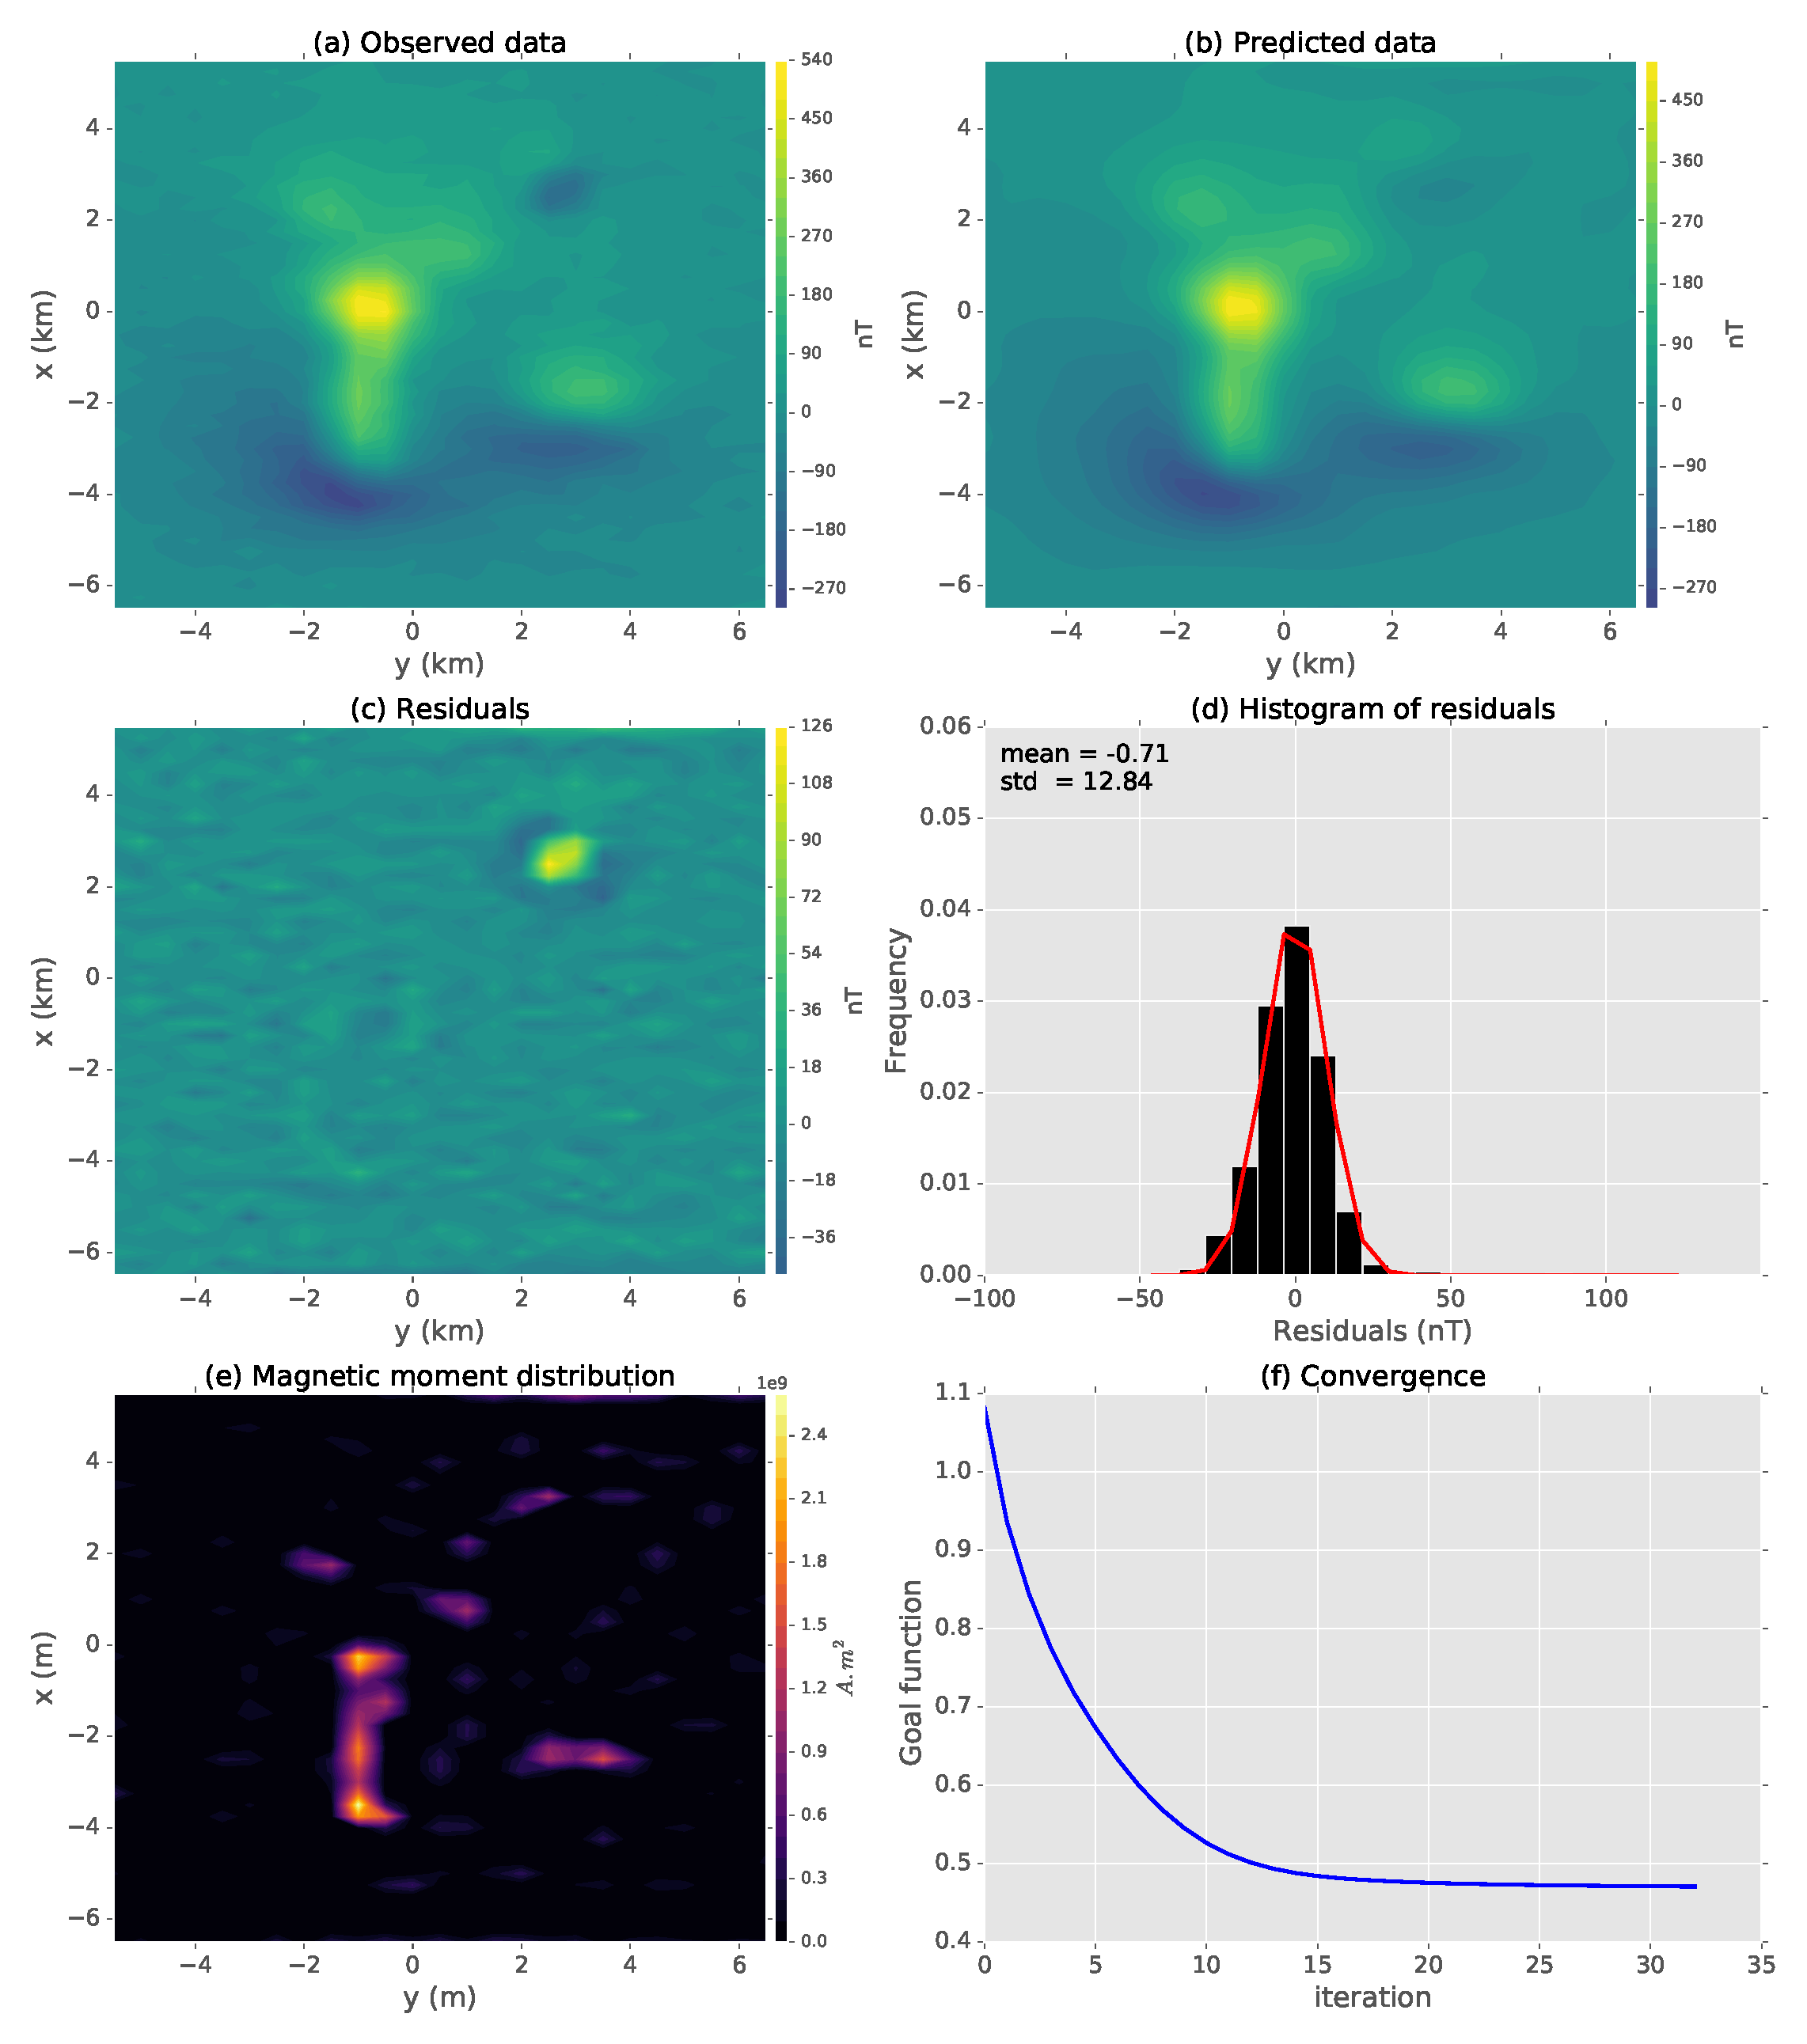
\includegraphics[width=0.85\textwidth]{Fig/unidir_shallow_diff_test/results_compiled_LM_NNLS_magRM.eps}
	\caption{Application to synthetic data with a shallow interfering source with different magnetization direction. (a) Noise-corrupted data. (b) Predicted data produced by equivalent layer. (c) Difference between the data shown in panels (a) and (b). (d) Histogram of residuals. (e) All-positive magnetic moment distribution. (f) Goal function value (equation \ref{eq:positivity_goal_function}a) per iteration showing the convergence.}
	\label{fig:unidir_shallow_diff_test}
\end{figure}

%% Real data application 
\begin{figure}
	\centering
	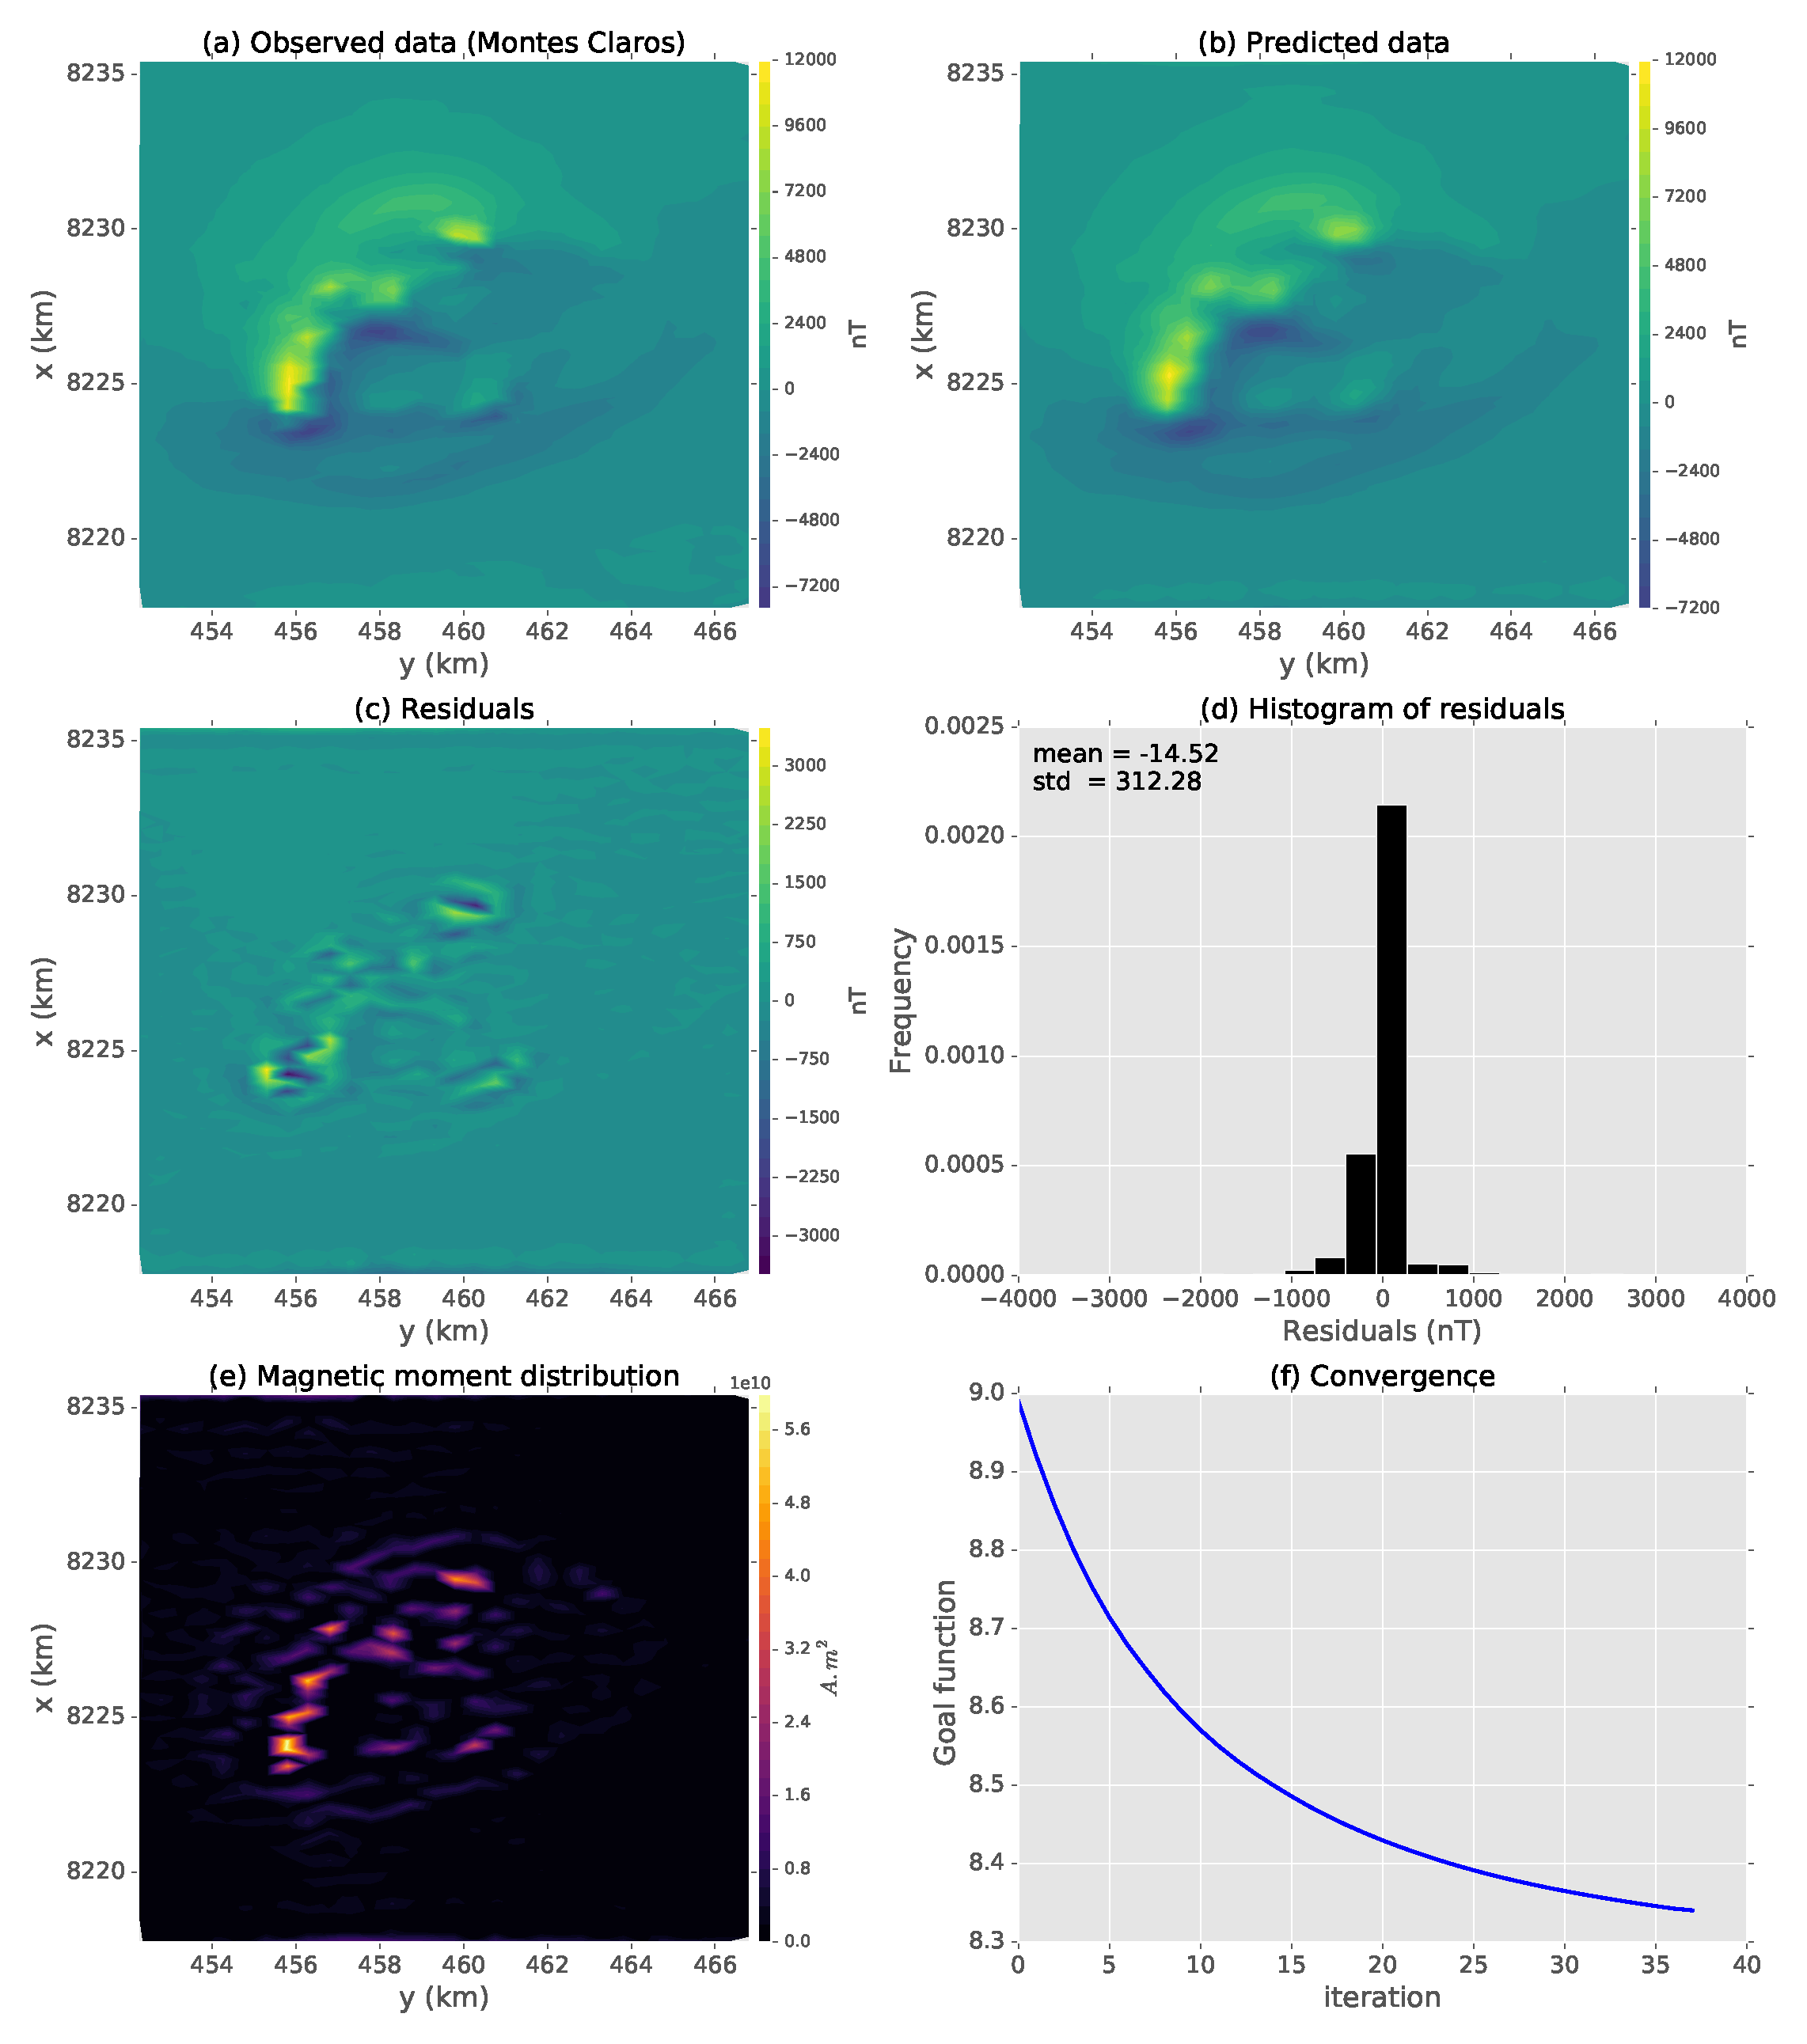
\includegraphics[width=0.85\textwidth]{Fig/field_data_montes_claros/montes_claros_compiled_LM_NNLS_magRM.eps}
	\caption{Application to field data located in complex of Montes Claros. (a) Observation data. (b) Predicted data produced by equivalent layer. (c) Difference between the data shown in panels (a) and (b). (d) Histogram of residuals. (e) All-positive magnetic moment distribution. (f) Goal function value (equation \ref{eq:positivity_goal_function}a) per iteration showing the convergence.}
	\label{fig:mc_data_application}
\end{figure}

\begin{figure}
	\centering
	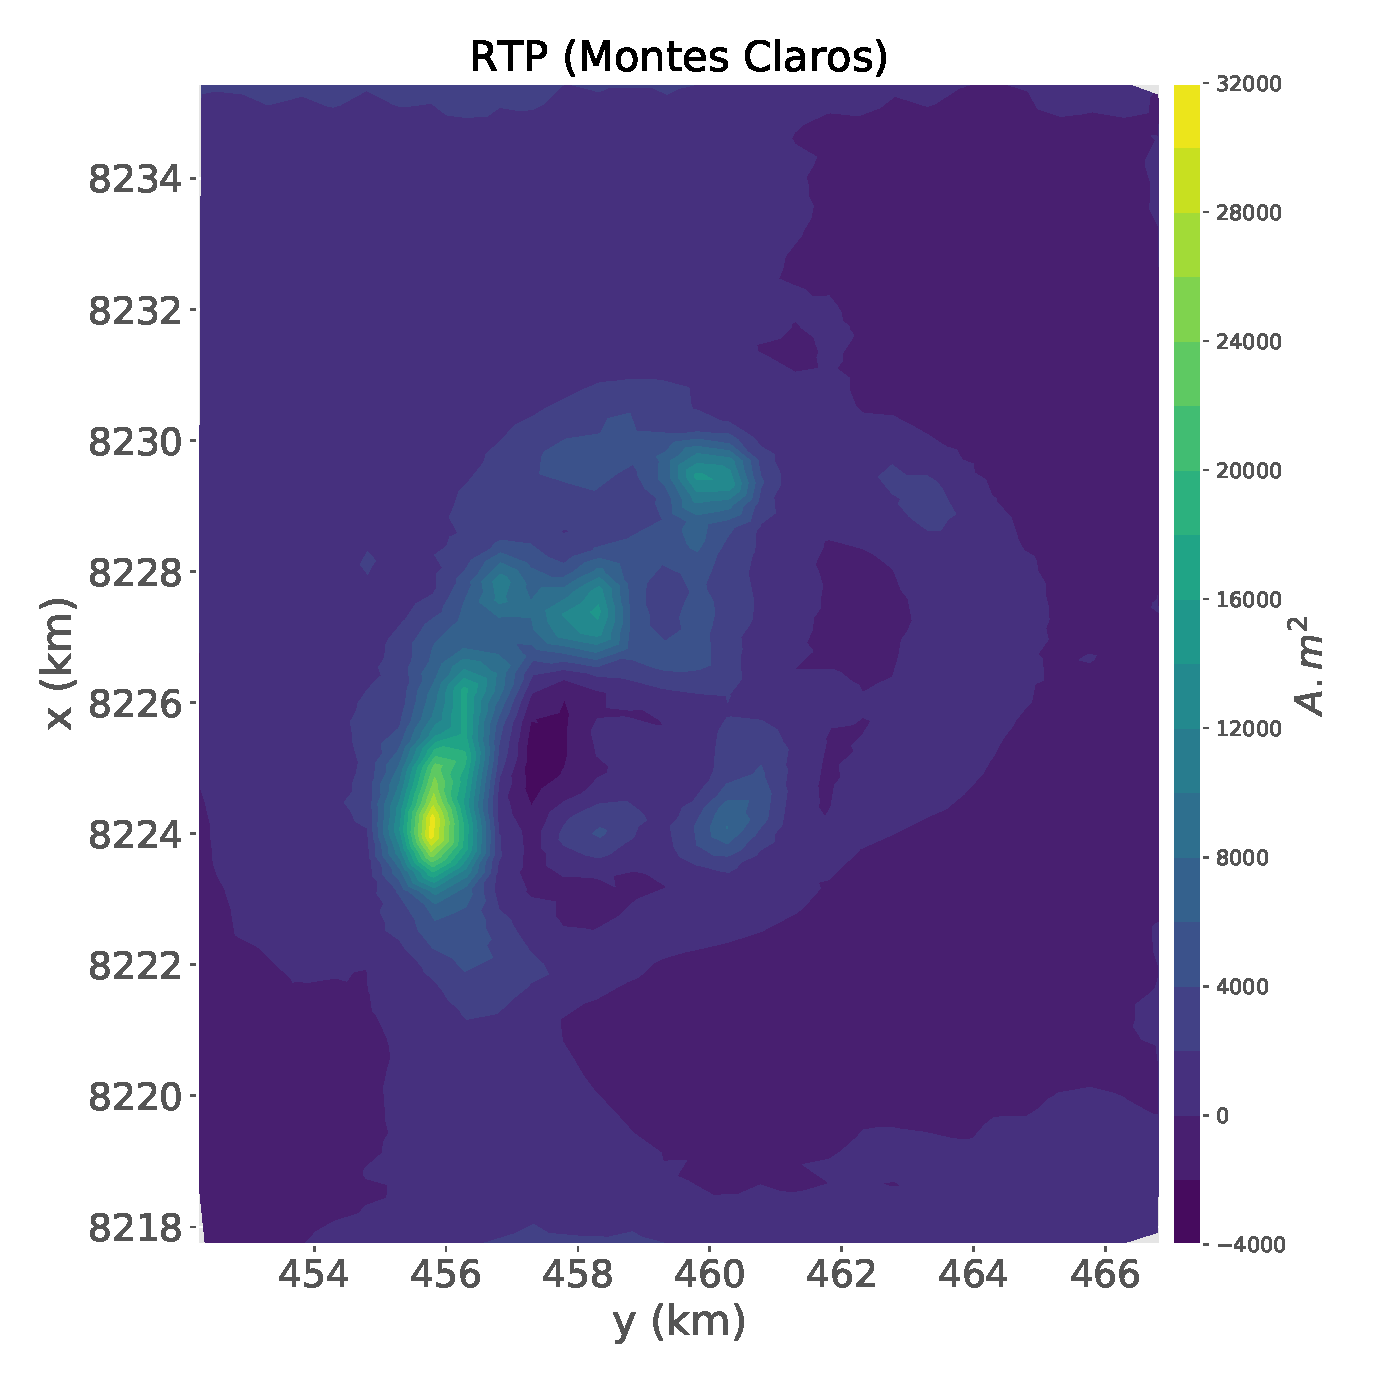
\includegraphics[width=0.75\textwidth]{Fig/field_data_montes_claros/RTP_data_montes_claros.eps}
	\caption{Application to field data located in complex of Montes Claros. RTP anomaly computed by using the estimated magnetization distribution shown in figure \ref{fig:mc_data_application}e.}
	\label{fig:rtp_mc_data}
\end{figure}



\end{document}
